\documentclass[11pt,a4paper]{article}
\usepackage[margin=18mm]{geometry}
\usepackage{amsmath,amssymb,mathtools}
\usepackage{booktabs,array,enumitem}
\usepackage[dvipsnames]{xcolor}
\usepackage{listings}
\usepackage{tikz}
\usetikzlibrary{arrows.meta,positioning,circuits.ee.IEC}
\usepackage[most]{tcolorbox}
\usepackage{hyperref}
\hypersetup{colorlinks=true,urlcolor=MidnightBlue,linkcolor=MidnightBlue}
\setlength{\parindent}{0pt}
\setlength{\parskip}{4pt}
\newcommand{\course}{Computational Methods in Physics}
\newtcolorbox{keybox}{colback=RoyalBlue!5,colframe=RoyalBlue!65!black,boxrule=.7pt,arc=2mm}
\newtcolorbox{checkbox}{colback=ForestGreen!5,colframe=ForestGreen!55!black,boxrule=.7pt,arc=2mm}
\newtcolorbox{aibox}{colback=BurntOrange!7,colframe=BurntOrange!80!black,boxrule=.7pt,arc=2mm}
\lstdefinestyle{matlabstyle}{
  language=Matlab,
  basicstyle=\ttfamily\footnotesize,
  keywordstyle=\color{RoyalBlue!75!black},
  commentstyle=\color{ForestGreen!55!black},
  stringstyle=\color{BurntOrange!80!black},
  numbers=left,
  numberstyle=\scriptsize\color{black!50},
  numbersep=5pt,
  frame=single,
  rulecolor=\color{RoyalBlue!25},
  backgroundcolor=\color{RoyalBlue!3},
  showstringspaces=false,
  columns=fullflexible,
  keepspaces=true,
  breaklines=true
}
\begin{document}

{\large\textsc{\course}}\\[-2pt]
{\small Learning Note \textbar\ Week 3}\par\vspace{4pt}
{\LARGE\bfseries Linear Systems Through Kirchhoff Circuits}\par\vspace{3pt}
\textit{A matrix is useful only after its rows have a clear physical origin and its solution survives independent checks.}

\begin{keybox}
\textbf{Physical question.} Can nodal and mesh analysis determine unknown voltages and currents while making every equation, unit, sign convention, and validation check defensible?
\end{keybox}

\section*{Learning outcomes}
By the end of this week, you should be able to:
\begin{enumerate}[nosep,leftmargin=5mm]
  \item define circuit unknowns and sign conventions before calculation;
  \item derive Kirchhoff equations before assembling $\mathbf{A}\mathbf{x}=\mathbf{b}$;
  \item preserve units while interpreting matrix rows, columns, and solutions;
  \item solve a square linear system with MATLAB's backslash operator;
  \item use rank, conditioning, residuals, Kirchhoff balances, and power balance as distinct evidence; and
  \item identify bounded physical problem spaces for a later capstone investigation.
\end{enumerate}

\section*{1. From a physical network to a linear system}
Many physical models produce several equations that must be satisfied simultaneously. Circuit currents and voltages, force balances, coupled static displacements, calibration equations, and conservation constraints can all take the form
\begin{equation}
  \mathbf{A}\mathbf{x}=\mathbf{b}.
\end{equation}
The matrix is not the model by itself. Each row must come from a stated physical law, each column must correspond to one declared unknown, and every term within an equation must have compatible units.

\begin{center}
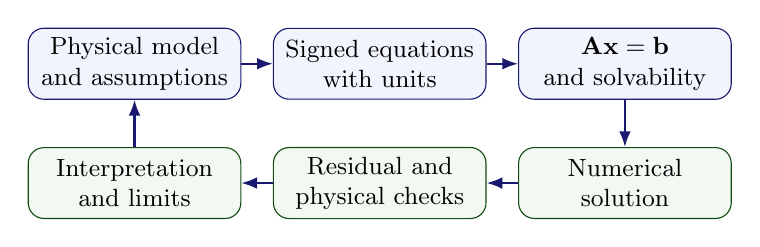
\begin{tikzpicture}[node distance=6mm and 4mm,every node/.style={font=\small,align=center},box/.style={draw=MidnightBlue,rounded corners=2mm,fill=RoyalBlue!7,minimum width=27mm,minimum height=9mm},test/.style={draw=ForestGreen!55!black,rounded corners=2mm,fill=ForestGreen!6,minimum width=27mm,minimum height=9mm},arrow/.style={-{Latex[length=2mm]},thick,MidnightBlue}]
\node[box] (m) {Physical model\\and assumptions};
\node[box,right=of m] (e) {Signed equations\\with units};
\node[box,right=of e] (a) {$\mathbf{A}\mathbf{x}=\mathbf{b}$\\and solvability};
\node[test,below=of a] (s) {Numerical\\solution};
\node[test,left=of s] (v) {Residual and\\physical checks};
\node[test,left=of v] (i) {Interpretation\\and limits};
\draw[arrow] (m)--(e); \draw[arrow] (e)--(a); \draw[arrow] (a)--(s);
\draw[arrow] (s)--(v); \draw[arrow] (v)--(i); \draw[arrow] (i)--(m);
\end{tikzpicture}
\end{center}

\section*{2. Worked model: two-node resistive network}
A $12.0\,\mathrm{V}$ ideal source feeds node A through $R_1=4.0\,\Omega$. Node A connects to ground through $R_2=6.0\,\Omega$ and to node B through $R_3=5.0\,\Omega$. Node B connects to ground through $R_4=10.0\,\Omega$.

Assume ideal wires, steady DC conditions, constant ohmic resistors, and zero voltage at ground. The unknowns are the node voltages
\begin{equation}
  \mathbf{v}=\begin{bmatrix}V_A\\V_B\end{bmatrix}.
\end{equation}
Branch currents are positive from the first named point toward the second.

\begin{checkbox}
\textbf{Predict before computing.} Without solving, predict the ordering of $V_s$, $V_A$, $V_B$, and ground. Then predict the current direction in every resistor. A numerical answer that violates this ordering requires diagnosis even if MATLAB reports no error.
\end{checkbox}

\section*{3. Derive Kirchhoff equations before assembling the matrix}
At node A, current entering from the source equals current leaving toward ground and node B:
\begin{equation}
  \frac{V_s-V_A}{R_1}=\frac{V_A}{R_2}+\frac{V_A-V_B}{R_3}.
\end{equation}
At node B,
\begin{equation}
  \frac{V_A-V_B}{R_3}=\frac{V_B}{R_4}.
\end{equation}
Rearranging gives
\begin{equation}
\underbrace{\begin{bmatrix}
\frac1{R_1}+\frac1{R_2}+\frac1{R_3} & -\frac1{R_3}\\[2mm]
-\frac1{R_3} & \frac1{R_3}+\frac1{R_4}
\end{bmatrix}}_{\mathbf{G}\;(\mathrm{S})}
\underbrace{\begin{bmatrix}V_A\\V_B\end{bmatrix}}_{\mathbf{v}\;(\mathrm{V})}
=
\underbrace{\begin{bmatrix}V_s/R_1\\0\end{bmatrix}}_{\mathbf{i}\;(\mathrm{A})}.
\end{equation}
Because siemens times volts gives amperes, the units are consistent. The negative off-diagonal terms encode current shared between the two nodes; they are not arbitrary signs to memorise.

\section*{4. Inspect solvability before solving}
For a square $n\times n$ system, full rank means $\operatorname{rank}(\mathbf{A})=n$ and establishes a unique algebraic solution. A zero determinant also signals singularity for a square matrix, but rank generalises more directly.

The condition number $\kappa(\mathbf{A})$ estimates possible amplification of relative perturbations. A moderate condition number does not prove accuracy; a large value warns that uncertain inputs or round-off may strongly affect the solution.

\begin{center}
\small
\begin{tabular}{>{\raggedright\arraybackslash}p{.22\linewidth}>{\raggedright\arraybackslash}p{.34\linewidth}>{\raggedright\arraybackslash}p{.34\linewidth}}
\toprule
\textbf{Evidence} & \textbf{Question answered} & \textbf{Important limitation}\\ \midrule
Rank & Is a unique algebraic solution available? & Does not validate the physical model\\
Condition number & Is the solution potentially sensitive? & Does not measure the actual modelling error\\
Residual & Does the computed result satisfy the assembled equations? & Can be small for the wrong equations\\
Physical checks & Does the result satisfy independent expectations? & Each check has its own blind spots\\ \bottomrule
\end{tabular}
\end{center}

\section*{5. Solve with MATLAB and reconstruct the physics}
Use the backslash operator rather than an explicit inverse:
\begin{lstlisting}[style=matlabstyle,caption={Nodal-analysis system and solution}]
G_S = [1/R1_ohm + 1/R2_ohm + 1/R3_ohm, -1/R3_ohm;
       -1/R3_ohm, 1/R3_ohm + 1/R4_ohm];
i_A = [sourceVoltage_V/R1_ohm; 0];

assert(rank(G_S) == size(G_S,1))
conditionNumber = cond(G_S);
nodeVoltage_V = G_S\i_A;
VA_V = nodeVoltage_V(1);
VB_V = nodeVoltage_V(2);
\end{lstlisting}
The baseline result is
\begin{equation}
  V_A=6.20690\,\mathrm{V}, \qquad V_B=4.13793\,\mathrm{V}.
\end{equation}
Reconstruct the branch currents:
\begin{align}
 I_{s\to A}&=(V_s-V_A)/R_1=1.44828\,\mathrm{A},\\
 I_{A\to g}&=V_A/R_2=1.03448\,\mathrm{A},\\
 I_{A\to B}&=(V_A-V_B)/R_3=0.413793\,\mathrm{A},\\
 I_{B\to g}&=V_B/R_4=0.413793\,\mathrm{A}.
\end{align}
The positive values agree with the predicted directions, and $12>V_A>V_B>0$.

\section*{6. Layer algebraic and physical validation}
The algebraic residual is
\begin{equation}
  \mathbf{r}=\mathbf{G}\mathbf{v}-\mathbf{i}.
\end{equation}
A scaled residual avoids judging a dimensional vector using an unexplained absolute threshold:
\begin{lstlisting}[style=matlabstyle]
residual_A = G_S*nodeVoltage_V - i_A;
scaledResidual = norm(residual_A,inf) / ...
    (norm(G_S,inf)*norm(nodeVoltage_V,inf) + norm(i_A,inf));
\end{lstlisting}

Then return to the circuit. KCL requires
\begin{align}
 I_{s\to A}-I_{A\to g}-I_{A\to B}&=0,\\
 I_{A\to B}-I_{B\to g}&=0.
\end{align}
Power balance provides an independent whole-network check:
\begin{equation}
  V_sI_{s\to A}=I_{s\to A}^2R_1+I_{A\to g}^2R_2+I_{A\to B}^2R_3+I_{B\to g}^2R_4.
\end{equation}

\begin{aibox}
\textbf{Caution: a small residual is not physical proof.} If the matrix was assembled from the wrong sign convention, the computed solution can satisfy that wrong matrix extremely well. Always reconstruct the original conservation laws and apply at least one independent physical expectation.
\end{aibox}

\section*{7. Conditioning and sensitivity are different from residual}
If $R_4$ becomes extremely large, node B is weakly connected to ground. The matrix can become more sensitive even while the direct solve produces a tiny residual. This is not a contradiction:
\begin{itemize}[nosep,leftmargin=5mm]
  \item residual asks whether the computed solution satisfies the supplied equations;
  \item conditioning asks how much the solution could respond to perturbations in those equations; and
  \item modelling uncertainty asks whether the resistor values and ideal assumptions represent the real circuit.
\end{itemize}
Use a controlled parameter perturbation to observe sensitivity rather than interpreting the condition number as an error percentage.

\section*{8. Practical transfer: two-loop mesh currents}
The practical uses two clockwise mesh currents. The left loop contains $V_1=12\,\mathrm{V}$ and $R_1=4\,\Omega$; the right loop contains $V_2=5\,\mathrm{V}$ and $R_2=6\,\Omega$; the loops share $R_3=3\,\Omega$. Kirchhoff's voltage law gives
\begin{equation}
\begin{bmatrix}R_1+R_3&-R_3\\-R_3&R_2+R_3\end{bmatrix}
\begin{bmatrix}I_1\\I_2\end{bmatrix}
=\begin{bmatrix}V_1\\V_2\end{bmatrix}.
\end{equation}
The reference currents are $I_1=2.27778\,\mathrm{A}$, $I_2=1.31481\,\mathrm{A}$, and $I_1-I_2=0.962963\,\mathrm{A}$ through the shared resistor in the left-loop direction.

Strong evidence includes full rank, a moderate condition number, a scaled residual, independently reconstructed KVL balances, current-sign interpretation, and equality of source and resistor powers.

\section*{9. Capstone problem spaces begin with evidence}
A capstone question should be open enough to investigate but bounded enough to validate. Candidate spaces include:
\begin{center}
\small
\begin{tabular}{>{\raggedright\arraybackslash}p{.27\linewidth}>{\raggedright\arraybackslash}p{.29\linewidth}>{\raggedright\arraybackslash}p{.33\linewidth}}
\toprule
\textbf{Problem space} & \textbf{Possible output} & \textbf{Possible validation}\\ \midrule
Circuit or sensor network & node voltages, currents, calibration values & conservation, residual, reference component\\
Coupled physical modes & mode frequencies and shapes & symmetry, limiting case, orthogonality\\
Equilibrium or threshold & physically meaningful root & bracketing, residual, limiting behaviour\\
Motion or decay & trajectory or population history & convergence, conservation, analytic case\\
Experimental fitting & parameters and uncertainty & units, residual structure, held-out data\\
Random transport & distribution or scaling law & uncertainty, sample-size convergence\\ \bottomrule
\end{tabular}
\end{center}
This week, record candidate questions and validation evidence. Final topic selection comes later.

\begin{aibox}
\textbf{Responsible AI use.} AI may help translate already-derived equations into code or propose checks. Record what was accepted, modified, or rejected. Independently verify the equations, units, signs, rank, residual, conservation laws, and physical interpretation.
\end{aibox}

\section*{Three takeaways}
\begin{enumerate}[nosep,leftmargin=6mm]
  \item Derive and label physical equations before assembling a matrix.
  \item Rank, conditioning, and residual answer different questions; none replaces physical validation.
  \item A credible solution returns to the circuit through Kirchhoff balances, plausible signs and scales, and power conservation.
\end{enumerate}

\begin{keybox}
\textbf{Preparation for the practical.} Complete the Week 03 Individual Practical Check --- Quiz in Google Classroom when the lecturer confirms it is available. Then derive the two mesh equations, solve with backslash, defend the residual and physical checks, investigate controlled changes, and record two bounded capstone candidate questions.
\end{keybox}

\end{document}
